\pgfsetplotmarksize{0pt}
\begin{figure}
 \centering
 \caption{\label{fl_conv1}FLClustered/test1.txt},
 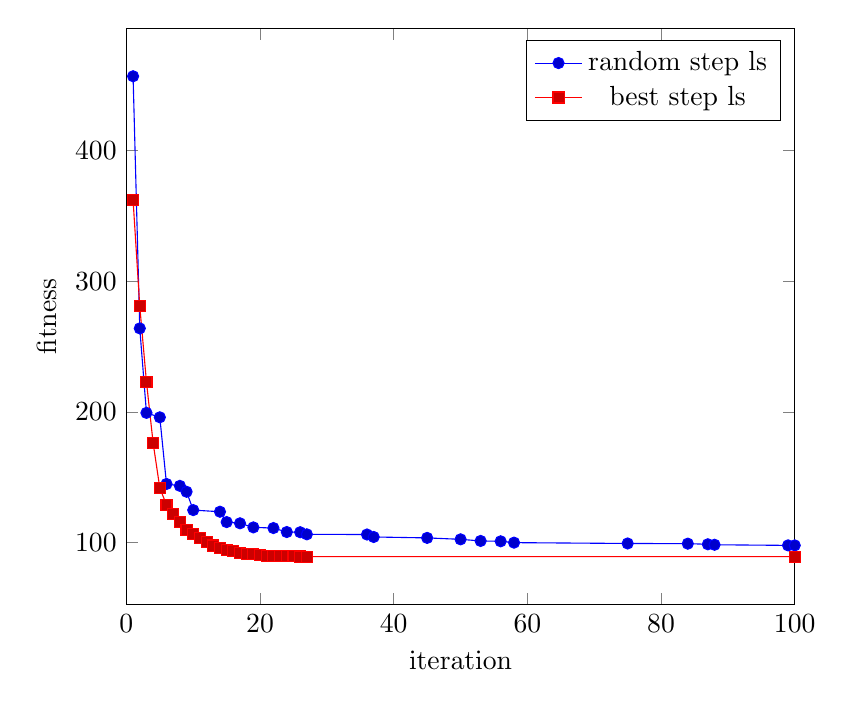
\begin{tikzpicture}
 \begin{axis}[
   width=0.7\textwidth,
   scale only axis,
   xlabel=iteration,
   ylabel=fitness,
   xmin=0,xmax=100,
   domain=0:100]
   \addplot coordinates {
     (0,inf)
     (1,456.8)
     (2,263.903)
     (3,199.258)
     (5,195.856)
     (6,144.86)
     (8,143.405)
     (9,138.894)
     (10,124.862)
     (14,123.616)
     (15,115.693)
     (17,114.756)
     (19,111.638)
     (22,111.127)
     (24,108.067)
     (26,107.936)
     (27,106.323)
     (36,106.186)
     (37,104.298)
     (45,103.591)
     (50,102.495)
     (53,101.26)
     (56,100.988)
     (58,99.9677)
     (75,99.3264)
     (84,99.1826)
     (87,98.7136)
     (88,98.3331)
     (99,97.8678)
     (100,97.8678)
   };
   \addlegendentry{random step ls}
   \addplot coordinates {
     (0,inf)
     (1,361.915)
     (2,280.809)
     (3,222.997)
     (4,176.132)
     (5,141.725)
     (6,128.923)
     (7,121.941)
     (8,115.628)
     (9,109.808)
     (10,106.445)
     (11,103.413)
     (12,100.411)
     (13,97.7217)
     (14,96.0056)
     (15,94.5528)
     (16,93.259)
     (17,92.1707)
     (18,91.4179)
     (19,90.9603)
     (20,90.5186)
     (21,90.0219)
     (22,89.8026)
     (23,89.6022)
     (24,89.5093)
     (25,89.4379)
     (26,89.3062)
     (27,89.2687)
     (100,89.2687)
   };
   \addlegendentry{best step ls}
 \end{axis}
 \end{tikzpicture}
\end{figure}
